\chapter{Teori}
I det følgende kapitel er en kort beskrivelse af 3D scanning - Struktureret Lys, og de principper metoden anvender. Sidst i kapitlet er der en kort introduktion til  Archimedes princip. 

\section{Fotogrammetri - struktureret lys}
3D-billedbehandling referer til teknikker som giver reel 3D data af et objekt. Der findes flere metoder som kan dette, valget af metode er afhængig af hvilken data der ønskes. Struktureret lys metoden er en metode der anvender en projektor samt et eller flere kameraer, hvor projektøren sender et struktureret lys på det emnet der ønskes information om. Metoden samler data om emnets overflade, hvilket kan andvendes til flere formål, som f.eks. volumenberegning og 3D printing. I denne rapport bliver struktureret lys andvendt til at lave volumenberegninger på permafrostkerner.
% Struktureret lys er en form for overfladeafbildning af et objekt, hvor punkter på objektets overflade bliver illustreret i et koordinatsystem (x,y,z).
% Hvor z-koordinaterne er en fuktion af (x,y) koordinaterne i et kartesiske koordinatsystem, og kan udtrykkes i matrice form som:
% ${z_{ij}=(x_i,y_j,)i=1,2...,L,j=1,2...,M}$.
Ved 3D-billedbehandlings system er det muligt at erhverve en skalar-værdi som en reflekterende overflade, associeret med et punkt på den ikke-plane overflade, hvilket resulterer i en punkt-sky der beskrives ved: $P_i=(x_i,y_i,z_i,f_i),i=1,2...,N$, hvor $f_i$ repræsenterer værdien af overfladepunktet i, i data sættet. Ligeledes repræsenteres farver ved: $P_i=(x_i,y_i,z_i,r_i,g_i,b_i),i=1,2...,N$, hvor vektorene $r_i$,$g_i$ og $b_i$ repræsenterer farvene illustreret på figur \vref{fig:opst_strukt_lys} (rød, grøn og blå), i det givne overfladepunkt (i). 
Ved struktureret lys metoden belyses et objektet med et specielt designet 2D rumligt varierende mønster, som vist på figur \vref{fig:opst_strukt_lys}, hvor den rumligt varierende 2D struktureret belysning genereret af en projektor designet til det formål, eller en anden lyskilde moduleret af en rumlig lysmodulator (Geng,2011).

Intensiteten af hvert piksel på det strukturerede lys-mønster er repræsenteret av et digitalt signal: $I_{ij}=(i,j),i=1,2,...,I,j=1,2,...,J$, hvor (i,j) repræsenterer (x,y) koordinaterne til det projekterende mønster.
En billede sensor som f.eks. et kamera anvendes til at optage 2D bilede af det strukturerede lys. Hvis det er tale om en plan overflade uden 3D variation, er det strukturede mønster fanget af kamera ens med det projekterende lys. Hvis der er tale om et rumlig objekt, vil overfladen af objektet forvrænge det projekterende lys, der fanges af kameraet. Princippet ved strukturered lys 3D billedbehandlingssytem er at indsamle 3D information fra det forvrængede lys.Geometrienaf objektet kalkuleres ved brug af struktureret lys principper og algoritmer. Ved brug af triangulering kan det geometriske forhold mellem bildesensoren (kamera), projektor og hvert enkelt punktet på objektets overflade, se figur \vref{fig:opst_strukt_lys}, kan udtrykkes ved formel: \vref{eq:triangulering_kam} (Geng,2011). 

%
\begin{equation}
R=B*\frac{sin(\theta)}{sin(\alpha+\theta)}
\label{eq:triangulering_kam}
\end{equation}
%


%Struktureret lys skanning, er en form for fotogrammetri som er en alsidig metode til at opnåelse af 3D form. Almindelige kameraer kan kun optage 2D, da de mangler dybde information. Ved struktureret lys metoden, anvendes der samtidig en projektor der lægger et mønster over det objekt der ønsker information om.  

\begin{figure}
\centering
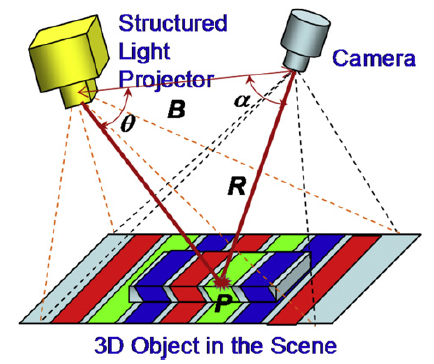
\includegraphics[width=0.6\textwidth]{Unavngivet}
\caption{Opstilling-struktureret lys (Geng,2011).}
\label{fig:opst_strukt_lys}
\end{figure}
  

% %
% \begin{figure}
% \centering
% %%%% BEGIN DOCUMENT
%\begin{document}
%
%
%
%

\begin{tikzpicture}
%%%% -----------Stativ + holder-------------%%%%
% \draw [gray, ultra thick]	(-4,-4) -- (-2,-4)	 			;		
% \draw [gray, ultra thick]	(-3,-4) -- (-3,4)	 			;		
% \draw [gray, ultra thick]	(-3,4) -- (1,4)					;
% \draw [gray, ultra thick]	(1,4) -- (1,0)					;
% \draw [black, ultra thick]	(1,0) -- (0,-2)					;
% \draw [black, ultra thick]	(1,0) -- (2,-2)					;
% \draw [black, ultra thick]	(0,-2) -- (2,-2)					;

%%%----------Vægt---------%%%
% \draw [gray, ultra thick]	(0,-2.7) -- (2,-2.7)			;
% \draw [gray, ultra thick]	(0,-2.7) -- (0,-2.9)			;

% \draw [gray, ultra thick]	(-0.5,-2.9) -- (2.5,-2.9)		;
% \draw [gray, ultra thick]	(2.0,-2.7) -- (2.0,-2.9)		;
% \draw [gray, ultra thick]	(-0.5,-2.9) -- (2.5,-2.9)		;

% \draw [gray, ultra thick]	(-0.5,-4) -- (3.5,-4)			;
% \draw [gray, ultra thick]	(-0.5,-2.9) -- (-0.5,-4.0)		;
% \draw [gray, ultra thick]	(2.5,-2.9) -- (3.5,-4)			;
% \node at (1.0,-3.5) {Vægt} 									;


%%%%------------Prøve----------------%%	
\draw[red, ultra thick, pattern=north east lines, pattern color=gray] (1.0,-2) circle [radius=0.5] ;
% \draw [red, ultra thick] (1.0,1.5) circle [radius=0.5]		;
\node [right] at (4.0,-2) {Prøveemne}						;
\draw [->] (3.9,-2) -- (2.0,-2);
%%%%------------Beholder Isobar----------------%%	
\draw [black, ultra thick]	(-0.5,0.5) -- (-0.5,-2.5)	 		;	
\draw [black, ultra thick]	(2.5,0.5) -- (2.5,-2.5)	 			;
\draw [black, ultra thick]	(-0.5,-2.5) -- (2.5,-2.5)	 		;
% \node at (1.0,-1.0) {Isopar} ;
\node [right] at (4.0,-1){Beholder}			 ;
\draw [->] (3.9, -1) -- (2.7,-1)							 ;



%%%-------------Kurve-------------%%%
% \draw[ultra thick, blue]
%     (-0.5,0.0) sin (-0.25,0.25) cos(0.0,0) sin (0.25,-0.25) cos(0.5,0.0) sin(0.75,0.25) cos(1,0.0) sin(1.25,-0.25) cos(1.5,0.0) sin(1.75,0.25) cos(2.0,0.0) sin(2.25,-0.25) cos(2.5,0.0);

 \draw[dashed, thick, blue] 
	(-0.5,0) -- (2.5,0)	;
 \draw[ultra thick,blue] 
 (-0.5,0.25) -- (2.5,0.25)	;
% \node [above] at (-1.5,2) {Temperaturføler}		;

% %%%-----------Føler-----------%%%
% %\draw [green, thick] (-0.0,-1) -- (-0.0,-2.5);
% \draw[gray, dashed] (-0.25,-0.5) -- (-0.25,0.5);
% \draw[gray, dashed] (-0.25,0.5) to [out=90, in = 0] (-2,2)		;

% \draw [ultra thick, green] (-0.25,-0.5) -- (-0.25,-1.5) 		;
   

% \node [left,black] at (-4,-4) {$L_1$}							;
% \node [right,black] at (1.5,1.5) {$L_2$}						;
% \node [below left,black] at (-2,1) {$d_{1,1}$}				;
% \node [above right,black] at (2,-1) {$d_{1,2}$}				;
% \node [below right,black] at (1.25,1.25) {$d_{2,1}$}						;
% \node [above left,black] at (-0.25,-0.25) {$d_{2,2}$}			;

%%%---------- Hjelpe linjer ------------%%%

%   \draw [help lines] (-5,-5) grid (5,5);
%   \draw [help lines, step = 2,ultra thick] (-5,-0) grid (5,0);
%   \draw [help lines, step = 2,ultra thick] (-0,-5) grid (0,5);
%%%%%
\end{tikzpicture}



%\end{document}
% \caption{Nedsænkning af et legeme i en væske}
% \label{fig:arki_ops_veske_teori}
% \end{figure}
% %

\section{Opdrift og Archimedes princip}
Archimedes princip omhandler kræfters påvirkning af et legeme ned-sænket i en væske. Et legeme nedsænket i væske påvirkes af tyngdekraften $F_g$ samt en opadrettet kraft (opdrift) $F_o$, hvor opdriften, svarer til vægten af den fortrængte væske, $m_for$, dette under forudsætning at væsken ikke er i bevægelse. 
Ved at nedsænke et legeme med en kendt masse og volumen, kan en væskes densitet bestemmes. Når væskens densitet kendes, kan volumen bestemmes af et hvilket som helst legeme såfremt det nedsænkes i den samme væske, under samme forhold.(Fishbane et al. 1996) 

Når et legeme flyder højt, som i figur \vref{fig:arki_fop} gælder fælgende forudsætniger: 
%
\begin{equation} 
 V^\prime< V
\end{equation}
% 
% 
\begin{equation} 
 F_o=\rho_v*V^\prime=F_g=\rho*V
\end{equation}
% 
% 
\begin{equation} 
 \frac{V^\prime}{V}=\frac{\rho}{\rho_v}
\end{equation}
% 
Hvor $V^\prime$ er det fortrængte volumen, $F_g$ er gravitation, $F_o$ er opdrift, $V$ er objektets totale volumen, $\rho_v$ er væskens densitet, og den totale kraft der påvirker objektet $F_{tot}=0$. 
%
\begin{figure}
\centering
%%%% BEGIN DOCUMENT
%\begin{document}
%
%
%
%

\begin{tikzpicture}

%%%%------------Prøve----------------%%	
\draw[red, ultra thick, pattern=north east lines, pattern color=gray] (1.0,0) circle [radius=0.5] ;
% \draw [red, ultra thick] (1.0,1.5) circle [radius=0.5]		;
\node [right] at (4.0,0.25) {Prøveemne}						;
\draw [->] (3.9,0.25) -- (1.7,0.25)								;
\node [left] at (0.25,0.8) {$\mathbf{{F}_{o}}$}			;
\draw [ultra thick][->] (0.4,0.1)--(0.4,1)				;
\node [left] at (0.25,-0.8) {$\mathbf{{F}_{g}}$}			;
\draw [ultra thick][->] (0.4,-0.1)--(0.4,-1.0)				;

%%%%------------Beholder Isobar----------------%%	
\draw [black, ultra thick]	(-0.5,0.5) -- (-0.5,-2.5)	 		;	
\draw [black, ultra thick]	(2.5,0.5) -- (2.5,-2.5)	 			;
\draw [black, ultra thick]	(-0.5,-2.5) -- (2.5,-2.5)	 		;
% \node at (1.0,-1.0) {Isopar} ;
\node [right] at (4.0,-1){Beholder}			 ;
\draw [->] (3.9, -1) -- (2.7,-1)							 ;

% {$\mathbf{M}_{ji}$} (j)

%%%-------------Kurve-------------%%%

%  \draw[dashed, thick, blue] 
% 	(-0.5,0) -- (2.5,0)	;
 \draw[ultra thick,blue] 
 	(-0.5,0.0) -- (0.47,0.0)	;
 \draw[dashed, thick, blue] 
 	(0.5,0.0) -- (1.5,0)	;
 \draw[ultra thick,blue] 
 (1.53,0.0) -- (2.5,0.0)	;
\node [right] at (4.0,-2) {Væske}						;
\draw [->] (3.9,-2) -- (2.2,-2)								;


%%%---------- Hjelpe linjer ------------%%%

%    \draw [help lines] (-5,-5) grid (5,5);
%    \draw [help lines, step = 2,ultra thick] (-5,-0) grid (5,0);
%    \draw [help lines, step = 2,ultra thick] (-0,-5) grid (0,5);
%%%%%
\end{tikzpicture}

\caption{Legeme der flyder-$F_{tot}=op$}
\label{fig:arki_fop}
\end{figure}
%
For et legeme der flyder i overfladen som vist på figur \vref{fig:arki_foverflade}, gælder følgende principper:
% 
\begin{equation}
V^\prime=V
\end{equation}
%
% 
\begin{equation}
\rho=\rho_v
\end{equation}
% 
Hvor de to volumener og densitet er ens, og $F_{tot}=0$.
% 
% 
\begin{figure}
\centering
%%%% BEGIN DOCUMENT
%\begin{document}
%
%
%
%

\begin{tikzpicture}

%%%%------------Prøve----------------%%	
\draw[red, ultra thick, pattern=north east lines, pattern color=gray] (1.0,-0.5) circle [radius=0.5] ;
% \draw [red, ultra thick] (1.0,1.5) circle [radius=0.5]		;
\node [right] at (4.0,-0.5) {Prøveemne}						;
\draw [->] (3.9,-0.5) -- (1.7,-0.5)								;
\node [left] at (0.25,0.4) {$\mathbf{{F}_{o}}$}			;
\draw [ultra thick][->] (0.4,-0.4)--(0.4,0.5)				;
\node [left] at (0.25,-1.3) {$\mathbf{{F}_{g}}$}			;
\draw [ultra thick][->] (0.4,-0.6)--(0.4,-1.54)				;

%%%%------------Beholder Isobar----------------%%	
\draw [black, ultra thick]	(-0.5,0.5) -- (-0.5,-2.5)	 		;	
\draw [black, ultra thick]	(2.5,0.5) -- (2.5,-2.5)	 			;
\draw [black, ultra thick]	(-0.5,-2.5) -- (2.5,-2.5)	 		;
% \node at (1.0,-1.0) {Isopar} ;
\node [right] at (4.0,-1){Beholder}			 ;
\draw [->] (3.9, -1) -- (2.7,-1)							 ;

% {$\mathbf{M}_{ji}$} (j)

%%%-------------Kurve-------------%%%

%  \draw[dashed, thick, blue] 
% 	(-0.5,0) -- (2.5,0)	;
 \draw[ultra thick,blue] 
 	(-0.5,0.0) -- (2.5,0.0)	;
%  \draw[dashed, thick, blue] 
%  	(0.5,0.0) -- (1.5,0)	;
%  \draw[ultra thick,blue] 
%  (1.53,0.0) -- (2.5,0.0)	;
 \node [right] at (4.0,-2) {Væske}						;
 \draw [->] (3.9,-2) -- (2.2,-2)								;


%%%---------- Hjelpe linjer ------------%%%

%    \draw [help lines] (-5,-5) grid (5,5);
%    \draw [help lines, step = 2,ultra thick] (-5,-0) grid (5,0);
%    \draw [help lines, step = 2,ultra thick] (-0,-5) grid (0,5);
%%%%%
\end{tikzpicture}

\caption{Legeme nedsunken i væske - $F_{tot}=0$}
\label{fig:arki_foverflade}
\end{figure}
%
% 
Når objektet synker, eller er fuldstendig neddykket som vist på figur \vref{fig:arki_fdown} gælder følgende forudsætninger:

% 
\begin{equation}
V^\prime=V
\end{equation}
% 
% 
\begin{equation}
\rho>\rho_v
\end{equation}
% 
Volumen af den neddykede objekt er det samme som volumen af den fortrængte væske, densiteten af objektet er større en densiteten af væsken, hvilket medfører at objektet synker (Fishbane et al. 1996). 
%
\begin{figure}
\centering
%%%% BEGIN DOCUMENT
%\begin{document}
%
%
%
%

\begin{tikzpicture}

%%%%------------Prøve----------------%%	
\draw[red, ultra thick, pattern=north east lines, pattern color=gray] (1.0,-1) circle [radius=0.5] ;
% \draw [red, ultra thick] (1.0,1.5) circle [radius=0.5]		;
\node [right] at (4.0,-1) {Prøveemne}						;
\draw [->] (3.9,-1) -- (1.7,-1)								;
\node [left] at (0.25,-0.4) {$\mathbf{{F}_{o}}$}			;
\draw [ultra thick][->] (0.4,-0.9)--(0.4,-0.1)				;
\node [left] at (0.25,-1.4) {$\mathbf{{F}_{g}}$}			;
\draw [ultra thick][->] (0.4,-1.1)--(0.4,-1.9)				;

%%%%------------Beholder Isobar----------------%%	
\draw [black, ultra thick]	(-0.5,0.5) -- (-0.5,-2.5)	 		;	
\draw [black, ultra thick]	(2.5,0.5) -- (2.5,-2.5)	 			;
\draw [black, ultra thick]	(-0.5,-2.5) -- (2.5,-2.5)	 		;
% \node at (1.0,-1.0) {Isopar} ;
\node [right] at (4.0,-1.5){Beholder}			 ;
\draw [->] (3.9, -1.5) -- (2.7,-1.5)							 ;

% {$\mathbf{M}_{ji}$} (j)

%%%-------------Kurve-------------%%%

%  \draw[dashed, thick, blue] 
% 	(-0.5,0) -- (2.5,0)	;
 \draw[ultra thick,blue] 
 (-0.5,0.0) -- (2.5,0.0)	;
 \node [right] at (4.0,-2) {Væske}						;
\draw [->] (3.9,-2) -- (2.2,-2)								;



%%%---------- Hjelpe linjer ------------%%%

%    \draw [help lines] (-5,-5) grid (5,5);
%    \draw [help lines, step = 2,ultra thick] (-5,-0) grid (5,0);
%    \draw [help lines, step = 2,ultra thick] (-0,-5) grid (0,5);
%%%%%
\end{tikzpicture}

\caption{Legeme der synker-$F_{tot}=ned$}
\label{fig:arki_fdown}
\end{figure}
%